\chapter{Confronto tra i linguaggi (trovare un titolo adeguato)}

\section{Punti di forza e debolezze di Objective-C}
TODO
\section{Punti di forza e debolezze di Swift}
TODO
\section{Confronto delle performance e gestione della memoria}
Esistono due modalità di gestione della memoria:\\
\\-MMR (Manual retain-release), dove lo sviluppatore gestisce esplicitamente la memoria, tenendo traccia degli oggetti instanziati. E' implementato tramite un modello chiamato Reference Counting, fornito dalla classe NSObject in congiunzione all'ambiente di runtime; è il metodo più obsoleto e più dispendioso in termini di tempo di sviluppo in quanto è un approccio prettamente manuale.\\
\\-ARC (Automatic reference counting), che utilizza lo stesso sistema di tracciamento degli oggetti di MMR, ma aggiunge automaticamente chiamate ai metodi di gestione della memoria a tempo di compilazione. Questo sistema permette di assicurare che gli oggetti abbiano vita il tempo necessario per il loro utilizzo e non oltre, poichè il compilatore genera in automatico anche i metodi di dealloc appropriati.\\E' l'approccio moderno e più utilizzato della gestione della memoria in Objective-C e Swift.
\begin{figure}[H]
      \centering
      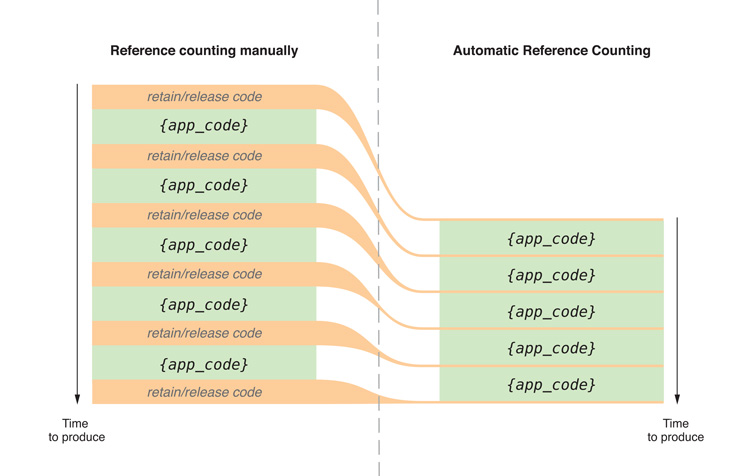
\includegraphics[scale=0.40]{immagini/ARC.jpg}
            \vspace{0.8cm}
            \caption{\textit{Confronto tra MMC ed ARC relativo al tempo di creazione dei cicli di retain-release degli oggetti}}
    \end{figure}
